\chapter{Retrieval augmented generation (RAG)}



\section{Information retrieval}

\begin{description}
    \item[Ad-hoc retrieval] \marginnote{Ad-hoc retrieval}
        Given a query, provide an ordered list of relevant documents from some (unstructured) collection.

        To determine relevancy, query and documents are embedded in some form and compared with a distance metric.

        \begin{figure}[H]
            \centering
            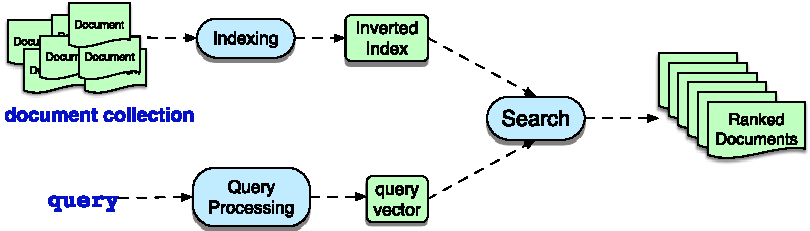
\includegraphics[width=0.75\linewidth]{./img/_info_retrieval.pdf}
        \end{figure}

    \item[Inverted index] \marginnote{Inverted index}
        Mapping from terms to documents with pre-computed term frequencies (and/or term positions). It allows narrowing down the document search space by considering only those that match the terms in the query.
\end{description}


\subsection{Document embeddings}

\begin{description}
    \item[TF-IDF embedding] \marginnote{TF-IDF embedding}
        Embed a document using the TF-IDF weighted term-document matrix.

        \begin{description}
            \item[Document scoring]
                Given a document $d$, a query $q$, and their respective embeddings $\vec{d}$ and $\vec{q}$, their similarity score is computed as their cosine similarity:
                \[
                    \begin{split}
                        \texttt{score}(q, d) &= \frac{\vec{q} \cdot \vec{d}}{|\vec{q}| \cdot |\vec{d}|} \\
                        &= \sum_{t \in q} \left( \frac{\texttt{tf-idf}(t, q)}{\sqrt{\sum_{q_i \in q} \texttt{tf-idf}^2(q_i, q)}} \cdot \frac{\texttt{tf-idf}(t, d)}{\sqrt{\sum_{d_i \in d} \texttt{tf-idf}^2(d_i, d)}} \right) \\
                    \end{split}
                \]
                As query terms tend to have count $1$ (i.e., $\forall t \in q: \texttt{tf-idf}(t, q) \approx \texttt{idf}(t)$, which is already present in $\texttt{tf-idf}(t, d)$), $\texttt{tf-idf}(t, q)$ can be dropped together with its normalization factor $|\vec{q}|$ (which is the same for all documents). Then, the score can be simplified and approximated to:
                \[ \texttt{score}(q, d) = \sum_{t \in q} \frac{\texttt{tf-idf}(t, d)}{|\vec{d}|} = \sum_{t \in q} \frac{\texttt{tf-idf}(t, d)}{\sqrt{\sum_{d_i \in d} \texttt{tf-idf}^2(d_i, d)}} \]

                \begin{example}
                    Given:
                    \begin{itemize}
                        \item The query $q = \texttt{sweet love}$,
                        \item The documents:
                        \[
                            \begin{split}
                                d_1 &= \texttt{sweet sweet nurse! love?} \\
                                d_2 &= \texttt{sweet sorrow} \\
                                d_3 &= \texttt{how sweet is love?} \\
                                d_4 &= \texttt{nurse!} \\
                            \end{split}
                        \]
                    \end{itemize}
                    The embeddings of $q$ and $d_1$ are computed as follows:
                    \begin{table}[H]
                        \centering
                        \footnotesize
                        \begin{tabular}{c|cccc|cccc}
                            \toprule
                            \textbf{Word} & \textbf{Count} & \texttt{tf} & \texttt{tf-idf} & $\texttt{tf-idf}/|q|$ & \textbf{Count} & \texttt{tf} & \texttt{tf-idf} & $\texttt{tf-idf}/|d_1|$ \\
                            \midrule
                            \texttt{sweet}  & $1$ & $1.000$ & $0.125$ & $0.383$ & $2$ & $1.301$ & $0.163$ & $0.357$ \\
                            \texttt{nurse}  & $0$ & $0$     & $0$     & $0$     & $1$ & $1.000$ & $0.301$ & $0.661$ \\
                            \texttt{love}   & $1$ & $1.000$ & $0.301$ & $0.924$ & $1$ & $1.000$ & $0.301$ & $0.661$ \\
                            \texttt{how}    & $0$ & $0$     & $0$     & $0$     & $0$ & $0$     & $0$     & $0$ \\
                            \texttt{sorrow} & $0$ & $0$     & $0$     & $0$     & $0$ & $0$     & $0$     & $0$ \\
                            \texttt{is}     & $0$ & $0$     & $0$     & $0$     & $0$ & $0$     & $0$     & $0$ \\
                            \midrule
                            & \multicolumn{4}{l|}{$|q| = \sqrt{0.125^2 + 0.301^2} = 0.326$} & \multicolumn{4}{l}{$|d_1| = \sqrt{0.163^2 + 0.301^2 + 0.301^2} = 0.456$} \\
                            \bottomrule
                        \end{tabular}
                    \end{table}
                    The overall score is therefore:
                    \[ \texttt{score}(q, d_1) = (0.383 \cdot 0.357) + (0.924 \cdot 0.610) = 0.137 + 0.610 = 0.747 \]

                    By using the simplified formula, we have that:
                    \begin{table}[H]
                        \centering
                        \footnotesize
                        \begin{tabular}{ccccc}
                            \toprule
                            \textbf{Document} & $|d_i|$ & $\texttt{tf-idf}(\texttt{sweet})$ & $\texttt{tf-idf}(\texttt{love})$ & \texttt{score} \\
                            \midrule
                            $d_1$ & $0.456$ & $0.163$ & $0.301$ & $1.017$ \\
                            $d_2$ & $0.615$ & $0.125$ & $0$ & $0.203$ \\
                            $d_3$ & $0.912$ & $0.125$ & $0.301$ & $0.467$ \\
                            $d_4$ & $0.301$ & $0$ & $0$ & $0$ \\
                            \bottomrule
                        \end{tabular}
                    \end{table}
                \end{example}
        \end{description}


    \item[Okapi BM25] \marginnote{Okapi BM25}
        TF-IDF variant with two additional parameters:
        \begin{itemize}
            \item $k$ to balance between \texttt{tf} and \texttt{idf},
            \item $b$ to weigh the importance of document length normalization.
        \end{itemize} 
        It is defined as follows:
        \[ 
            \texttt{BM25}(q, d) = 
                \sum_{t \in q} \left( \texttt{idf}(t) \frac{\texttt{tf}(t, d) \cdot (k+1)}{k \cdot \left( 1 - b + b \frac{|d|}{|d_\text{avg}|} \right) + \texttt{tf}(t, d)} \right)
        \]
        where $|d_\text{avg}|$ is the average document length, and typically $k \in [1.2, 2]$ and $b = 0.75$.


    \item[Dense embedding] \marginnote{Dense embedding}
        Embed a document using a pre-trained encoder (e.g., BERT).

        \begin{figure}[H]
            \centering
            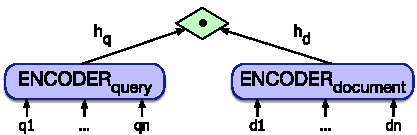
\includegraphics[width=0.45\linewidth]{./img/_info_retrieval_dense_embedding.pdf}
        \end{figure}

        \begin{description}
            \item[Document scoring]
                Use nearest neighbor with the dot product as distance. To speed-up search, approximate k-NN algorithms can be used.
        \end{description}
\end{description}


\subsection{Metrics}

\begin{description}
    \item[Precision/recall] \marginnote{Precision/recall}
        Given:
        \begin{itemize}
            \item The set of documents returned by the system $T$,
            \item The selected relevant documents $R \subseteq T$,
            \item The selected irrelevant documents $N \subseteq T$,
            \item All the relevant documents $U \supseteq R$.
        \end{itemize}
        Precision and recall are computed as:
        \[ 
            \texttt{precision} = \frac{|R|}{|T|} 
            \qquad
            \texttt{recall} = \frac{|R|}{|U|} 
        \]

    \item[Precision-recall curve] \marginnote{Precision-recall curve}
        Given a ranked list of documents, plot recall and precision by considering an increasing number of documents.

        \begin{description}
            \item[Interpolated precision]
                Smoothed version of the precision-recall curve.

                Consider recalls at fixed intervals and use as precision at position $r$ the maximum of all the next ones:
                \[ \texttt{precision}_\texttt{interpolated}(r) = \max_{i \geq r} \texttt{precision}(i) \]
        \end{description}

    \item[Average precision] \marginnote{Average precision}
        Average precision by considering the predictions up to a cut-off threshold $t$. Given the relevant documents $R_t$ in the first $t$ predictions, average precision is computed as:
        \[ \texttt{AP}_t = \frac{1}{|R_t|} \sum_{d \in R_t} \texttt{precision}_t(d) \]
        where $\texttt{precision}_t(d)$ is computed w.r.t. the position of the document $d$ in the ranked list.

        \begin{description}
            \item[Mean average precision] \marginnote{Mean average precision}
                Average AP over different queries $Q$:
                \[ \texttt{mAP}_t = \frac{1}{|Q|} \sum_{q \in Q} \texttt{AP}_t(q) \]
        \end{description}
\end{description}

\begin{example}
    Consider the following ranked predictions:
    \begin{table}[H]
        \centering
        \footnotesize
        \begin{tabular}[t]{cccc}
            \toprule
            \textbf{Rank} & \textbf{Relevant?} & \textbf{Precision}$_t$ & \textbf{Recall}$_t$ \\
            \midrule
            1  & Y & 1.0 & 0.11 \\
            2  & N & 0.50 & 0.11 \\
            3  & Y & 0.66 & 0.22 \\
            4  & N & 0.50 & 0.22 \\
            5  & Y & 0.60 & 0.33 \\
            6  & Y & 0.66 & 0.44 \\
            7  & N & 0.57 & 0.44 \\
            8  & Y & 0.63 & 0.55 \\
            9  & N & 0.55 & 0.55 \\
            10 & N & 0.50 & 0.55 \\
            11 & Y & 0.55 & 0.66 \\
            12 & N & 0.50 & 0.66 \\
            13 & N & 0.46 & 0.66 \\
            \bottomrule
        \end{tabular}
        \quad
        \begin{tabular}[t]{cccc}
            \toprule
            \textbf{Rank} & \textbf{Relevant?} & \textbf{Precision}$_t$ & \textbf{Recall}$_t$ \\
            \midrule
            14 & N & 0.43 & 0.66 \\
            15 & Y & 0.47 & 0.77 \\
            16 & N & 0.44 & 0.77 \\
            17 & N & 0.44 & 0.77 \\
            18 & Y & 0.44 & 0.88 \\
            19 & N & 0.42 & 0.88 \\
            20 & N & 0.40 & 0.88 \\
            21 & N & 0.38 & 0.88 \\
            22 & N & 0.36 & 0.88 \\
            23 & N & 0.35 & 0.88 \\
            24 & N & 0.33 & 0.88 \\
            25 & Y & 0.36 & 1.00 \\
            \bottomrule
        \end{tabular}
    \end{table}

    The precision-recall curve is the following:
    \begin{figure}[H]
        \centering
        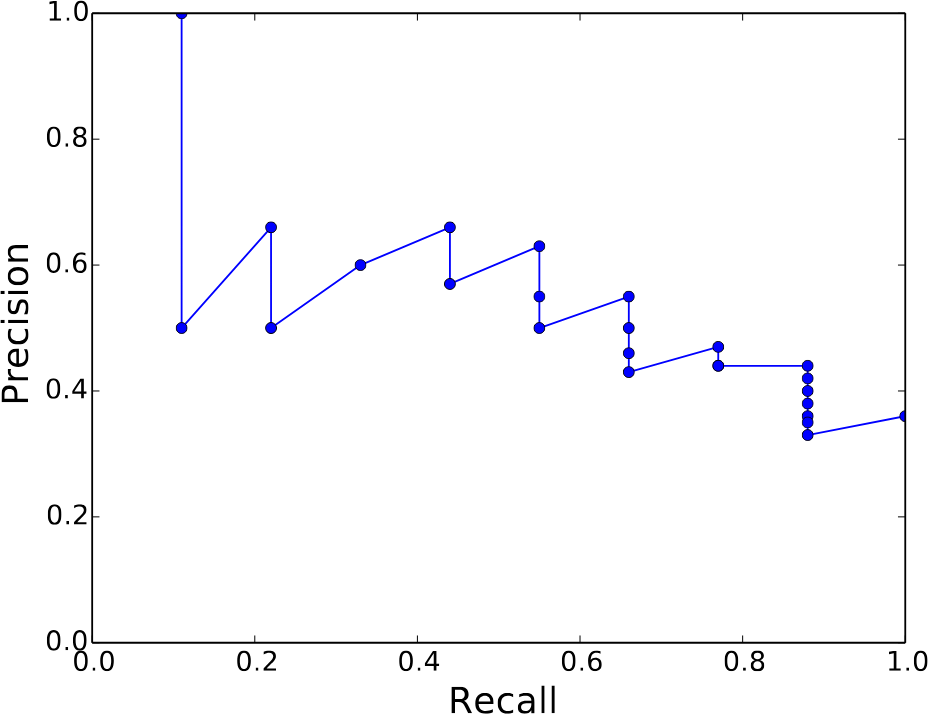
\includegraphics[width=0.4\linewidth]{./img/ir_pr_curve.png}
    \end{figure}
    Interpolated with $11$ equidistant recall points, the curve is:
    \begin{figure}[H]
        \centering
        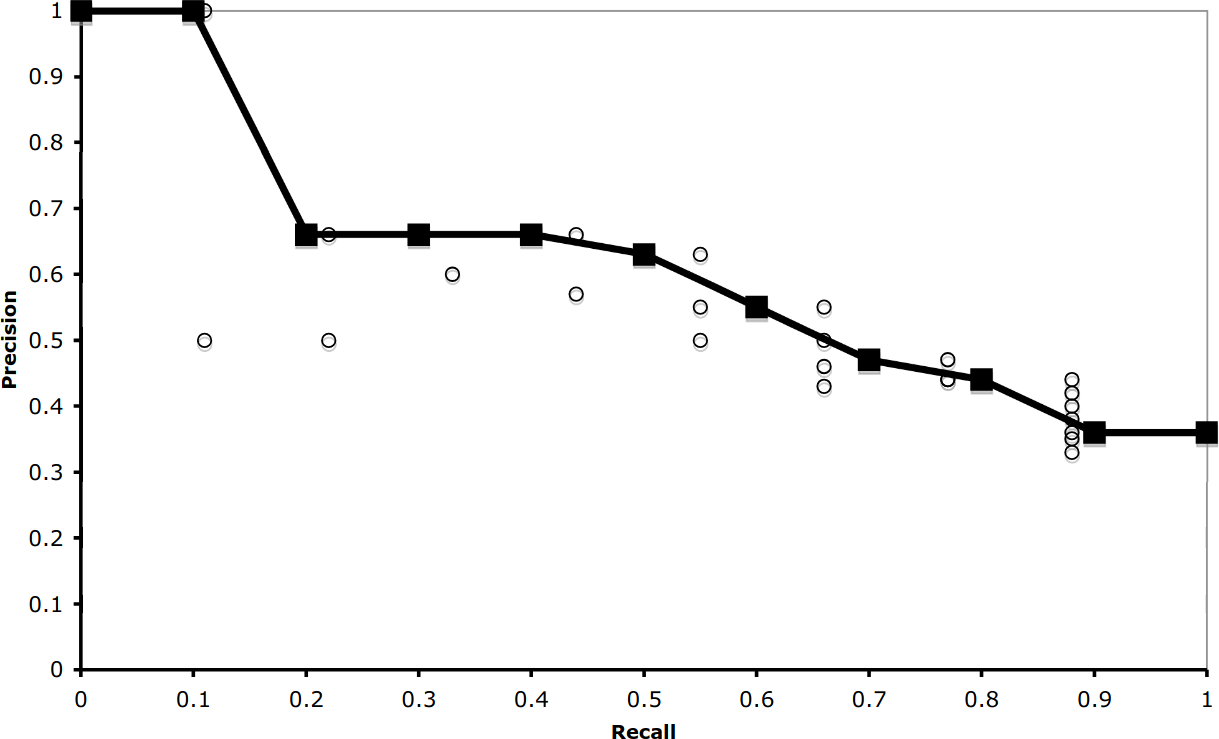
\includegraphics[width=0.45\linewidth]{./img/ir_pr_interpolated.png}
    \end{figure}

    Average precision computed over all the predictions (i.e., $t=25$) is:
    \[ \texttt{AP} = \frac{1.0 + 0.66 + 0.60 + 0.66 + 0.63 + 0.55 + 0.47 + 0.44 + 0.36}{9} = 0.6 \]
\end{example}



\section{Question answering}


\subsection{Reading comprehension task}

\begin{description}
    \item[Reading comprehension task] \marginnote{Reading comprehension task}
        Find a span of text in the document that answers a given question.

        More formally, given a question $q$ and a passage $p = p_1, \dots, p_m$, the following is computed for all tokens $p_i$:
        \begin{itemize}
            \item The probability $\mathcal{P}_\text{start}(i)$ that $p_i$ is the start of the answer span.
            \item The probability $\mathcal{P}_\text{end}(i)$ that $p_i$ is the end of the answer span.
        \end{itemize}

        \begin{figure}[H]
            \centering
            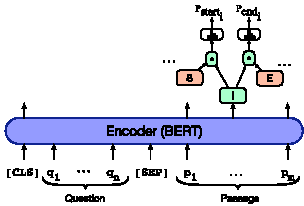
\includegraphics[width=0.35\linewidth]{./img/_qa_bert.pdf}
            \caption{Example of span labeling architecture}
        \end{figure}

        \begin{remark}
            A sliding window over the whole passage can be used if it is too long for the context length of the model.
        \end{remark}

        \begin{remark}
            The classification token \texttt{[CLS]} can be used to determine whether there is no answer.
        \end{remark}
\end{description}


\subsection{Metrics}

\begin{description}
    \item[Exact match] \marginnote{Exact match}
        Ratio of match between predicted answer and the ground-truth computed considering the characters at each position.

    \item[F1 score] \marginnote{F1 score}
        Macro F1 score computed by considering predictions and ground-truth as bag of tokens (i.e., average token overlap).

    \item[Mean reciprocal rank] \marginnote{Mean reciprocal rank}
        Given a system that provides a ranked list of answers to a question $q_i$, the reciprocal rank for $q_i$ is:
        \[ \texttt{RR} = \frac{1}{\texttt{rank}_i} \]
        where $\texttt{rank}_i$ is the index of the first correct answer in the provided ranked list.
        Mean reciprocal rank is computed over a set of queries $Q$:
        \[ \texttt{mRR} = \frac{1}{|Q|} \sum_{i=1}^{|Q|} \frac{1}{\texttt{rank}_i} \]

\end{description}


\subsection{Retrieval-augmented generation for question answering}

\begin{remark}
    Question answering with plain LLM prompting only is subject to the following problems:
    \begin{itemize}
        \item Hallucinations.
        \item It is limited to the training data and cannot integrate a new knowledge base.
        \item Its knowledge might not be up-to-date.
    \end{itemize}
\end{remark}

\begin{description}
    \item[RAG for QA] \marginnote{RAG for QA}
        Given a question and a collection of documents, the answer is generated in two steps by the following components:
        \begin{descriptionlist}
            \item[Retriever] 
                Given the question, it returns the relevant documents.

                \begin{remark}
                    The retriever should be optimized for recall.
                \end{remark}

                \begin{remark}
                    A more complex pipeline can be composed of:
                    \begin{descriptionlist}
                        \item[Rewriter] Rewrites the question into a better format.
                        \item[Retriever] Produces a ranked list of relevant documents.
                        \item[Reranker] Reorders the retrieved documents for a more fine-grained ranking.
                    \end{descriptionlist}
                \end{remark}

            \item[Reader] 
                Given the question and the relevant documents, it uses a backbone LLM to generate the answer through prompting.
        \end{descriptionlist}
\end{description}

\begin{remark}
    The current trend is to evaluate RAG performance with another LLM.
\end{remark}

\begin{remark}
    The collection of documents can also be a collection of passages or chunks of predetermined length.
\end{remark}

\begin{figure}[H]
    \centering
    \begin{subfigure}{0.75\linewidth}
        \centering
        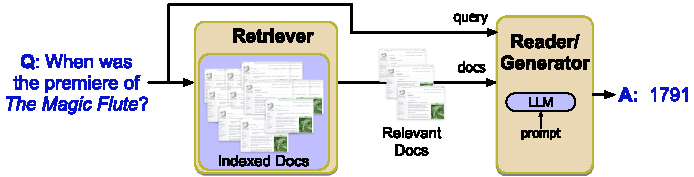
\includegraphics[width=\linewidth]{./img/_qa_rag1.pdf}
    \end{subfigure}
    \begin{subfigure}{0.9\linewidth}
        \centering
        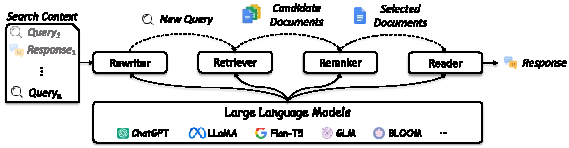
\includegraphics[width=\linewidth]{./img/_qa_rag2.pdf}
    \end{subfigure}
\end{figure}